%
%
% CSCI 1430 Written Question Template
%
% This is a LaTeX document. LaTeX is a markup language for producing documents. 
% You will fill out this document, compile it into a PDF document, then upload the PDF to Gradescope. 
%
% To compile into a PDF on department machines:
% > pdflatex thisfile.tex
%
% If you do not have LaTeX, your options are:
% - Personal laptops (all common OS): http://www.latex-project.org/get/ 
% - VSCode extension: https://marketplace.visualstudio.com/items?itemName=James-Yu.latex-workshop
% - Online Tool: https://www.overleaf.com/ - most LaTeX packages are pre-installed here (e.g., \usepackage{}).
%
% If you need help with LaTeX, please come to office hours.
% Or, there is plenty of help online:
% https://en.wikibooks.org/wiki/LaTeX
%
% Good luck!
% The CSCI 1430 staff
%
%%%%%%%%%%%%%%%%%%%%%%%%%%%%%%%%%%%%%%%%%%%%%%%%%%%%%%%%%%%%%%%%%%%%%
%
% How to include two graphics on the same line:
%
% \includegraphics[width=0.49\linewidth]{yourgraphic1.png}
% \includegraphics[width=0.49\linewidth]{yourgraphic2.png}
%
% How to include equations:
%
% \begin{equation}
% y = mx+c
% \end{equation}
%
% How to include code:
%
% \begin{python}
% def f(x):
%   return x
% \end{python}
%
%
%%%%%%%%%%%%%%%%%%%%%%%%%%%%%%%%%%%%%%%%%%%%%%%%%%%%%%%%%%%%%%%%%%%%%%%%%%%%%%%%%%%%%%%%%%%%%%%%

\documentclass[11pt]{article}

\usepackage[english]{babel}
\usepackage[utf8]{inputenc}
\usepackage{amsmath,amsfonts,amssymb,bm}
\usepackage{xcolor}
\usepackage[colorlinks = true,
            linkcolor = blue,
            urlcolor  = blue]{hyperref}
\usepackage[a4paper,margin=1.5in]{geometry}
\usepackage{stackengine,graphicx}
\usepackage{fancyhdr}
\setlength{\headheight}{15pt}
\usepackage{microtype}
\usepackage{times}
\usepackage[shortlabels]{enumitem}
\setlist[enumerate]{topsep=0pt}
\usepackage{framed}
\usepackage{mdframed}
\usepackage{xcolor}
\usepackage[most]{tcolorbox}
\usepackage{booktabs}

% a great python code format: https://github.com/olivierverdier/python-latex-highlighting
\usepackage{pythonhighlight}

\usepackage{trimclip,lipsum}

\frenchspacing
\setlength{\parindent}{0cm} % Default is 15pt.
\setlength{\parskip}{0.3cm plus1mm minus1mm}

\pagestyle{fancy}
\fancyhf{}
\lhead{Homework 3 Questions}
\rhead{CSCI 1430}
\lfoot{\textcolor{red}{\textbf{Only}
\ifcase\thepage
\or \textbf{instructions}
\or \textbf{Q1 (a)}
\or \textbf{Q1 (b)}
\or \textbf{Q1 (c)}
\or \textbf{Q1 (d)}
\or \textbf{Q2 (a) (i)}
\or \textbf{Q2 (a) (ii), (b)}
\or \textbf{Q2 (c)}
\or \textbf{Q2 (c)}
\or \textbf{Q2 (c)}
\or \textbf{Q3 (a)}
\or \textbf{Q3 (b)}
\or \textbf{Q4 (a)}
\or \textbf{Q4 (b)}
\or \textbf{feedback}
\else
\textbf{[ERROR: PAGE MISALIGNMENT]}
\fi
\textbf{should be on this page}
}}
\rfoot{\thepage/15}

\date{}

\title{\vspace{-1cm}Homework 3 Written Questions}


\begin{document}
\maketitle
\thispagestyle{fancy}

\section*{Template Instructions}

This document is a template with specific answer regions and a fixed number of pages. Given large class sizes and limited TA time, the template helps the course staff to grade efficiently and still focus on the content of your submissions. Please help us in this task:
 
\begin{itemize}
  \item Make this document anonymous.
  
  \item Questions are in the orange boxes. Provide answers in the green boxes.
  \item Use the footer to check for correct page alignment.

  \item \textbf{Do NOT remove the answer box.}
  \item \textbf{Do NOT change the size of the answer box.}
  \item \textbf{Extra pages are not permitted unless otherwise specified.}
  \item \textbf{Template edits or page misalignment will lead to a 10 point deduction.}
\end{itemize}

\section*{Gradescope Submission}
\begin{itemize}
  \item Compile this document to a PDF and submit it to Gradescope.
  \item Pages will be automatically assigned to the right questions on Gradescope.
\end{itemize}

\section*{This Homework}
\begin{itemize}
    \item 4 questions \textbf{[10 + 8 + 6 + 12 = 36 points]}.
    \item Include code, images, and equations where appropriate.
\end{itemize}

% Please leave the pagebreak
\pagebreak


%%%%%%%%%%%%%%%%%%%%%%%%%%%%%%%%%%%
\paragraph{Q1:} \textbf{[10 points]}
In 2D, suppose we have two quadrilaterals $ABCD$ and $A'B'C'D'$ as seen in the image below. They look like they might be related by a rotation and a non-uniform scale transformation.

Given the corresponding points, we will attempt to find $\bm{M}$ using linear least squares.

\begin{minipage}{0.5\linewidth}
    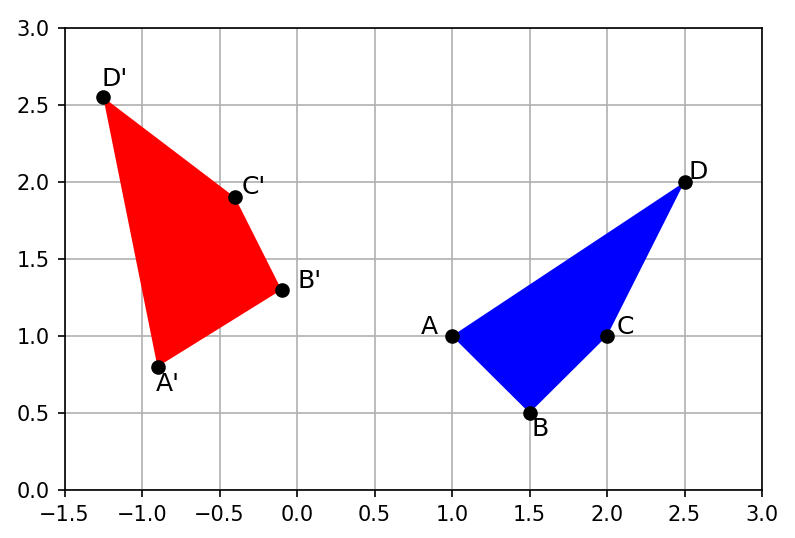
\includegraphics[width=\linewidth]{images/quads_lstsq.png}
\end{minipage}
\begin{minipage}{0.5\linewidth}
    \begin{equation}
    \begin{split}
    A&=(1, 1)\\
    B&=(1.5, 0.5)\\
    C&=(2, 1)\\
    D&=(2.5, 2)
    \end{split}
    \quad\quad\quad
    \begin{split}
    A'&=(-0.9, 0.8)\\
    B'&=(-0.1, 1.3)\\
    C'&=(-0.4, 1.9)\\
    D'&=(-1.25, 2.55)
    \end{split}
    \end{equation}
\end{minipage}

Let's try and map each point in $ABCD$ to its corresponding point in $A'B'C'D'$ by a $2\times2$ transformation matrix $\bm{M}$, as we know this can represent rotation and scale.

e.g. if $\bm{x} = \begin{pmatrix} x \\ y \end{pmatrix}$ and $\bm{x'} = \begin{pmatrix} x' \\ y' \end{pmatrix}$, and $\bm{M} = \begin{pmatrix} m_{1,1} & m_{1,2} \\ m_{2,1} & m_{2,2} \end{pmatrix}$

then $\begin{pmatrix} m_{1,1} & m_{1,2} \\ m_{2,1} & m_{2,2} \end{pmatrix} \times \begin{pmatrix} x \\ y \end{pmatrix} = \begin{pmatrix} x' \\ y'  \end{pmatrix}$

\begin{enumerate}[(a)]
\item \textbf{[2 point]} 
\begin{tcolorbox}[colback=orange!5!white,colframe=orange!75!black]
Rewrite $\bm{M}\bm{x} = \bm{x'}$ as a pair of linear equations by expanding the matrix multiplication. Define these algebraically with $x, y, x', y',$ or $0$.
\end{tcolorbox}

\begin{tcolorbox}[colback=white!5!white,colframe=green!75!black]
\setbox0=\hbox{\parbox[t]{\textwidth}{
    %%%%%%% ANSWER STARTS HERE %%%%%%%%%%%%%%%%%%%%%%%%%%%%

    TODO: Replace each of the `$\_\_$' below.
    \begin{align*}
    \begin{cases}
        \_\_m_{1,1} + \_\_m_{1,2} + \_\_m_{2,1} + \_\_m_{2,2} = \_\_
        \\\_\_m_{1,1} + \_\_m_{1,2} + \_\_m_{2,1} + \_\_m_{2,2} = \_\_
    \end{cases}
    \end{align*}

    %%%%%%% ANSWER ENDS HERE %%%%%%%%%%%%%%%%%%%%%%%%%%%%%%
    }}
\clipbox{0pt \dimexpr\dp0-4\baselineskip\relax{} 0in 0pt}{\copy0}
\end{tcolorbox}

\pagebreak
\item \textbf{[2 points]}
Systems of linear equations are denoted in the form $\bm{A}\bm{x} = \bm{b}$, where the vector $\bm{x}$ holds our entries of $\bm{M}$. 
To estimate the four parameters of $\bm{M}$, we will need four equations in our system such that it is \emph{determined}. 

But, as quadrilaterals have four points, we could form a system of eight equations (two for each point) that is said to be \emph{overdetermined}. In this case, it is possible to find values for $\bm{M}$ that minimize the distance (or residual error) between the approximated values for $X'$ and the real $X'$ values, i.e., that minimize $||\bm{A}\bm{x} - \bm{b}||_2$.

Form eight equations from the four $x$--$x'$, $y$--$y'$ correspondences, and construct a matrix $\bm{A}$ and column vector $\bm{b}$ that satisfy
\begin{align*}
    \bm{A} \times \begin{pmatrix} m_{1,1} \\ m_{1,2} \\ m_{2,1} \\ m_{2,2} \\ \end{pmatrix} = \bm{b}
\end{align*}

\begin{tcolorbox}[colback=orange!5!white,colframe=orange!75!black]
Declare $\bm{A}$ and $\bm{b}$:\\

Replace each of the `$\_\_$' below with a $0$ or a coordinate value from $ABCD$ and $A'B'C'D'$.
\end{tcolorbox}

\begin{tcolorbox}[colback=white!5!white,colframe=green!75!black]
\setbox0=\hbox{\parbox[t]{\textwidth}{
    %%%%%%% ANSWER STARTS HERE %%%%%%%%%%%%%%%%%%%%%%%%%%%%

    TODO: your answer for (b) here
    \begin{align*}
        \begin{pmatrix} 
        \_\_ & \_\_ & \_\_ & \_\_ \\ 
        \_\_ & \_\_ & \_\_ & \_\_ \\ 
        \_\_ & \_\_ & \_\_ & \_\_ \\ 
        \_\_ & \_\_ & \_\_ & \_\_ \\ 
        \_\_ & \_\_ & \_\_ & \_\_ \\ 
        \_\_ & \_\_ & \_\_ & \_\_ \\ 
        \_\_ & \_\_ & \_\_ & \_\_ \\ 
        \_\_ & \_\_ & \_\_ & \_\_
        \end{pmatrix} 
        \times \begin{pmatrix} m_{1,1} \\ m_{1,2} \\ m_{2,1} \\ m_{2,2} \\ \end{pmatrix} 
        = \begin{pmatrix} 
        \_\_ \\ 
        \_\_ \\ 
        \_\_ \\ 
        \_\_ \\ 
        \_\_ \\ 
        \_\_ \\ 
        \_\_ \\ 
        \_\_ 
        \end{pmatrix}
    \end{align*}

    %%%%%%% ANSWER ENDS HERE %%%%%%%%%%%%%%%%%%%%%%%%%%%%%%
    }}
\clipbox{0pt \dimexpr\dp0-10\baselineskip\relax{} 0in 0pt}{\copy0}
\end{tcolorbox}

\pagebreak
\item \textbf{[2 point]} To find a solution to our system, we need to invert $\bm{A}$ even though $\bm{A}$ is non-square. We can use the pseudoinverse of $\bm{A}$, written as $\bm{A}^+$. Left multiplying it by both sides gives us:
\begin{align*}
 \bm{A}^+ \bm{A}\bm{x} &= \bm{A}^+ \bm{b}\\
 \quad \bm{x} &= \bm{A}^+ \bm{b}.
\end{align*}

As long as $\bm{A}$ has a pseudoinverse, this solution minimizes $||\bm{A}\bm{x} - \bm{b}||_2$. This is the closed-form least squares solution, where $\bm{x} = (\bm{A}^\top \bm{A})^{-1}\bm{A}^\top\bm{b}$ and where $\bm{A}^+ = (\bm{A}^\top \bm{A})^{-1}\bm{A}^\top$.

We can compute the pseudoinverse from the singular value decomposition. In python, \texttt{numpy.linalg.lstsq()} will handle this for us. It takes as input $\bm{A}$ and $\bm{b}$, and returns a solution for $\bm{x}$ along with the residual error. Plug the values you wrote in part (c) into that function and write the returned $\bm{M}$ matrix here with the residual error.

\textit{Note:} You may need to reshape your output from \texttt{linalg.lstsq}.

\begin{tcolorbox}[colback=orange!5!white,colframe=orange!75!black]
Replace each `$\_\_$' below with the numeric value of $m_{i, j}$ and state the numeric value of the residual error:
\end{tcolorbox}

\begin{tcolorbox}[colback=white!5!white,colframe=green!75!black]
\setbox0=\hbox{\parbox[t]{\textwidth}{
    %%%%%%% ANSWER STARTS HERE %%%%%%%%%%%%%%%%%%%%%%%%%%%%
    Residual error: xxx
    \begin{align*}
        \bm{M} = \begin{pmatrix} m_{1,1} & m_{1,2} \\ m_{2,1} & m_{2,2} \end{pmatrix} = \begin{pmatrix} \_\_ & \_\_ \\ \_\_ & \_\_ \end{pmatrix}
    \end{align*}

    %%%%%%% ANSWER ENDS HERE %%%%%%%%%%%%%%%%%%%%%%%%%%%%%%
    }}
\clipbox{0pt \dimexpr\dp0-4\baselineskip\relax{} 0in 0pt}{\copy0}
\end{tcolorbox}

\pagebreak
\item \textbf{[4 point]} If the residual is zero (or zero to machine numerical precision), then we can confirm our initial hypothesis that the transformation is a rotation and a scale. If it is not, then we need a transformation with more degrees of freedom.

\begin{tcolorbox}[colback=orange!5!white,colframe=orange!75!black]
    Determine what kind of transformation it is by forming a system of linear equations and determining a matrix $\bm{M}$ that produces zero residual error (to machine numerical precision). 
    
    Write out your system's $\bm{A}$ and $\bm{b}$ matrices as in (b), state $\bm{M}$ and the residual as in (c), and state which kind of transformation it is.
\end{tcolorbox}

\begin{tcolorbox}[colback=white!5!white,colframe=green!75!black]
    \setbox0=\hbox{\parbox[t]{\textwidth}{
        %%%%%%% ANSWER STARTS HERE %%%%%%%%%%%%%%%%%%%%%%%%%%%%
        
    
        %%%%%%% ANSWER ENDS HERE %%%%%%%%%%%%%%%%%%%%%%%%%%%%%%
        }}
    \clipbox{0pt \dimexpr\dp0-24\baselineskip\relax{} 0in 0pt}{\copy0}
    \end{tcolorbox}

\end{enumerate}



%%%%%%%%%%%%%%%%%%%%%%%%%%%%%%%%%%%
% Please leave the pagebreak
\pagebreak
\paragraph{Q2:} \textbf{[8 points]}
In lecture, you've learned that cameras can be represented by intrinsic and extrinsic matrices. These matrices can be used to calculate the projections of points within a 3D world onto 2D image planes. For this, we use \emph{homogeneous coordinates}. The final $3\times4$ matrix is known as the \emph{camera matrix}.

Recall that the transformation can be represented by the following expression:
\begin{align*}
    \begin{pmatrix} 
    f_x & s & $0$ \\ 
    $0$ & f_y & $0$ \\ 
    $0$ & $0$ & $1$ \end{pmatrix} \times
    \begin{pmatrix} 
    r_{11} & r_{12} & r_{13} & t_x \\ 
    r_{21} & r_{22} & r_{23} & t_y \\  
    r_{31} & r_{32} & r_{33} & t_z
    \end{pmatrix} \times 
    \begin{pmatrix} 
    x \\ 
    y \\ 
    z \\ 
    $1$ \end{pmatrix}
    = w
    \begin{pmatrix}  u \\ v \\ $1$ \end{pmatrix}
\end{align*}
where $f$ is the focal point, $r$ is the rotation matrix, $t$ is the translation vector,  $w$ is some weighing/scaling factor, and $(u, v)$ is the position of the point in the real world $(x, y, z)$ projected on the 2D plane.

\begin{enumerate}[(a)]
\item \textbf{[2 points]}
For each of the following, you are given the camera specifications and a sample 3D point from the real world. 

\begin{tcolorbox}[colback=orange!5!white,colframe=orange!75!black]
Fill in the camera's intrinsic and extrinsic matrices; then, perform the multiplications and perspective division (unhomogenize) to find the 2D coordinate of the projected point on the image.
\end{tcolorbox}

\begin{enumerate} [(i)]
\item A camera with a focal length of 1 in both the $x$ and $y$ directions, a translation of 5 along the $x$-axis, and no skew or rotation.


\begin{tcolorbox}[colback=white!5!white,colframe=green!75!black]
\setbox0=\hbox{\parbox[t]{\textwidth}{
    %%%%%%% ANSWER STARTS HERE %%%%%%%%%%%%%%%%%%%%%%%%%%%%

    TODO: Fill in the \_\_ entries
    \begin{align*}
        & \qquad M_{\text{intrinsic}} \quad \times \qquad M_{\text{extrinsic}} \qquad  \times \; 
        \begin{pmatrix} 
            x  \\ 
            y  \\ 
            z  \\
            1
        \end{pmatrix} \\
        &= \begin{pmatrix} 
        \_\_ & \_\_ & $0$    \\  % <----- TODO: replace \_\_ %
        $0$ & \_\_ & $0$     \\  % <----- TODO: replace \_\_ %
        $0$ & $0$ & $1$ 
        \end{pmatrix} 
        \times
        \begin{pmatrix} 
        \_\_ & \_\_ & \_\_ & \_\_  \\ % <----- TODO: replace \_\_ %
        \_\_ & \_\_ & \_\_ & \_\_  \\ % <----- TODO: replace \_\_ %
        \_\_ & \_\_ & \_\_ & \_\_     % <----- TODO: replace \_\_ %
        \end{pmatrix} \times
        \begin{pmatrix} 
        $30$    \\ 
        $-20$   \\ 
        $10$    \\ 
        $1$ \end{pmatrix} \\
        &= \qquad \qquad \qquad \begin{pmatrix} 
        \_\_    \\   % <----- TODO: replace \_\_ %
        \_\_    \\   % <----- TODO: replace \_\_ %
        \_\_         % <----- TODO: replace \_\_ %
        \end{pmatrix} \\
        &= \qquad \quad \quad 
        \_\_         % <----- TODO: replace \_\_ %
        \times 
        \begin{pmatrix}  
        \_\_    \\   % <----- TODO: replace \_\_ %
        \_\_    \\   % <----- TODO: replace \_\_ %
        $1$ 
        \end{pmatrix}
    \end{align*}

    %%%%%%% ANSWER ENDS HERE %%%%%%%%%%%%%%%%%%%%%%%%%%%%%%
    }}
\clipbox{0pt \dimexpr\dp0-16\baselineskip\relax{} 0in 0pt}{\copy0}
\end{tcolorbox}

\pagebreak
\item A camera with focal length of $2$ in both the $x$ and $y$ directions, a translation of $5$ along the $x$-axis, and no skew or rotation.
\begin{tcolorbox}[colback=white!5!white,colframe=green!75!black]
\setbox0=\hbox{\parbox[t]{\textwidth}{
    %%%%%%% ANSWER STARTS HERE %%%%%%%%%%%%%%%%%%%%%%%%%%%%

    TODO: Fill in the \_\_ entries
    \begin{align*}
        &= \begin{pmatrix} 
        \_\_ & \_\_ & $0$    \\  % <----- TODO: replace \_\_ %
        $0$ & \_\_ & $0$     \\  % <----- TODO: replace \_\_ %
        $0$ & $0$ & $1$ 
        \end{pmatrix} 
        \times
        \begin{pmatrix} 
        \_\_ & \_\_ & \_\_ & \_\_  \\ % <----- TODO: replace \_\_ %
        \_\_ & \_\_ & \_\_ & \_\_  \\ % <----- TODO: replace \_\_ %
        \_\_ & \_\_ & \_\_ & \_\_     % <----- TODO: replace \_\_ %
        \end{pmatrix} \times
        \begin{pmatrix} 
        $30$    \\ 
        $-20$   \\ 
        $10$    \\ 
        $1$ \end{pmatrix} \\
        &= \qquad \qquad \qquad \begin{pmatrix} 
        \_\_    \\   % <----- TODO: replace \_\_ %
        \_\_    \\   % <----- TODO: replace \_\_ %
        \_\_         % <----- TODO: replace \_\_ %
        \end{pmatrix} \\
        &= \qquad \quad \quad 
        \_\_         % <----- TODO: replace \_\_ %
        \times 
        \begin{pmatrix}  
        \_\_    \\   % <----- TODO: replace \_\_ %
        \_\_    \\   % <----- TODO: replace \_\_ %
        $1$ 
        \end{pmatrix}
    \end{align*}

    %%%%%%% ANSWER ENDS HERE %%%%%%%%%%%%%%%%%%%%%%%%%%%%%%
    }}
\clipbox{0pt \dimexpr\dp0-12\baselineskip\relax{} 0in 0pt}{\copy0}
\end{tcolorbox}

\end{enumerate}
\item \textbf{[2 points]}

\begin{tcolorbox}[colback=orange!5!white,colframe=orange!75!black]
Compare the two image coordinates you've calculated in parts a and b. Explain how each parameter affects the final image coordinate. \textbf{[2-3 sentences]}
\end{tcolorbox}

\begin{tcolorbox}[colback=white!5!white,colframe=green!75!black]
\setbox0=\hbox{\parbox[t]{\textwidth}{
    %%%%%%% ANSWER STARTS HERE %%%%%%%%%%%%%%%%%%%%%%%%%%%%

    TODO: Your answer to (b) here.

    %%%%%%% ANSWER ENDS HERE %%%%%%%%%%%%%%%%%%%%%%%%%%%%%%
    }}
\clipbox{0pt \dimexpr\dp0-12\baselineskip\relax{} 0in 0pt}{\copy0}
\end{tcolorbox}

%%%%%%%%%%%%%%%%%%%%%%%%%%%%%%%%%%%
% \paragraph{A4a:} Your answer here.
% Uncomment the stencil below and fill in your solution.

% \begin{enumerate}[(a)]

% \item

% \end{enumerate}

% \begin{enumerate}[(b)]

% \item

% \begin{python}
% # Your code here
% \end{python}

% \includegraphics[width=0.5\linewidth]{yourscreenshot.png}

% \end{enumerate}

%%%%%%%%%%%%%%%%%%%%%%%%%%%%%%%%%%%
% Please leave the pagebreak
\pagebreak
\item \textbf{[4 points]}
In the questions folder, we've provided stencil code for a camera simulation in \texttt{camera\_simulation.py}. Given a camera matrix and a set of world points, the simulator visualizes an image that a camera would produce. 

\begin{tcolorbox}[colback=orange!5!white,colframe=orange!75!black]
Please implement \texttt{calculate\_camera\_matrix()} by calculating the camera matrix using the parameters given in the code (see stencil for more detail). When successful, you will see a bunny rendered as dots (see below). Paste your code for this function and attach a screenshot of the working demo once you finish. Play around with the sliders to see how different parameters affect the projection!
\end{tcolorbox}

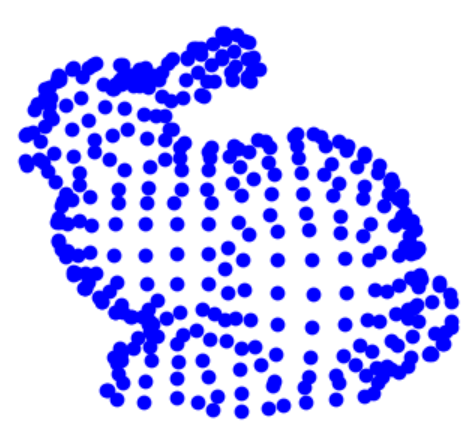
\includegraphics[width=0.5\linewidth]{images/bunny.png}

\begin{tcolorbox}[enhanced jigsaw,breakable,pad at break*=1mm,colback=white!5!white,colframe=green!75!black,height fixed for=all]
    %%%%%%% ANSWER STARTS HERE %%%%%%%%%%%%%%%%%%%%%%%%%%%%

    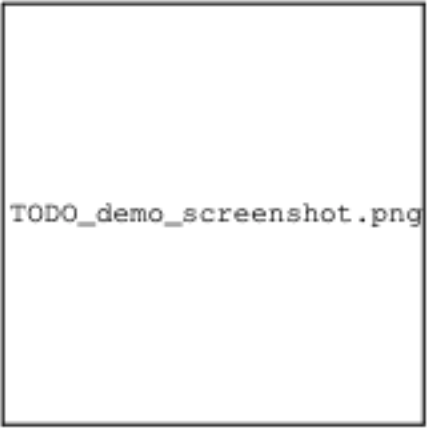
\includegraphics[width=0.5\textwidth,height=7cm,keepaspectratio]{images/TODO_demo_screenshot.png}


    \begin{python}
import numpy as np
import matplotlib.pyplot as plt
from mpl_toolkits import mplot3d
from matplotlib.widgets import Slider, Button

# Initial random matrices
initial_intrinsic_matrix_to_replace = np.random.rand(3,3)
initial_extrinsic_matrix_to_replace = np.random.rand(3,4)
initial_camera_matrix_to_replace = np.random.rand(3,4)

# Setting up the point cloud
file_data_path= "./images/bunny.xyz"
point_cloud = np.loadtxt(file_data_path, skiprows=0, max_rows=1000000)
# center it
point_cloud -= np.mean(point_cloud,axis=0)
# homogenize
point_cloud = np.concatenate((point_cloud, np.ones((point_cloud.shape[0], 1))), axis=1)
# move it in front of the camera
point_cloud += np.array([0,0,-0.15,0])

def calculate_camera_matrix(tx, ty, tz, alpha, beta, gamma, fx, fy, skew, u, v):
    """
    This function should calculate the camera matrix using the given
    intrinsic and extrinsic camera parameters.
    We recommend starting with calculating the intrinsic matrix (refer to lecture 8).
    Then calculate the rotational 3x3 matrix by calculating each axis separately and
    multiply them together.
    Finally multiply the intrinsic and extrinsic matrices to obtain the camera matrix.
    :params tx, ty, tz: Camera translation from origin
    :param alpha, beta, gamma: rotation about the x, y, and z axes respectively
    :param fx, fy: focal length of camera
    :param skew: camera's skew
    :param u, v: image center coordinates
    :return: [3 x 4] NumPy array of the camera matrix, [3 x 4] NumPy array of the intrinsic matrix, [3 x 4] NumPy array of the extrinsic matrix
    """
    ########################
    # TODO: Your code here #
    # Hint: Calculate the rotation matrices for the x, y, and z axes separately.
    # Then multiply them to get the rotational part of the extrinsic matrix.
    ########################
    return (initial_camera_matrix_to_replace, 
    initial_intrinsic_matrix_to_replace, 
    initial_extrinsic_matrix_to_replace)

def find_coords(camera_matrix):
    """
    This function calculates the coordinates given the student's calculated camera matrix.
    Normalizes the coordinates.
    Already implemented.
    """
    coords = np.matmul(camera_matrix, point_cloud.T)
    return coords / coords[2]













    ################################################
    # YOU MAY USE THIS ADDITIONAL PAGE

    # WARNING: IF YOU DON'T END UP USING THIS PAGE
    # KEEP THESE COMMENTS TO MAINTAIN PAGE ALIGNMENT
    ################################################
    \end{python}
    %%%%%%% ANSWER ENDS HERE %%%%%%%%%%%%%%%%%%%%%%%%%%%%
\end{tcolorbox}

% \begin{tcolorbox}[colback=white!5!white,colframe=green!75!black]
%     \clipbox{0pt \dimexpr\dp0-1\baselineskip\relax{} 0in 0pt}{\copy0}
% \end{tcolorbox}


% \paragraph{A4b:} Your answer here.



%%%%%%%%%%%%%%%%%%%%%%%%%%%%%%%%%%%
\pagebreak
\paragraph{Q3:} \textbf{[6 points]} Given a stereo pair of cameras:
\begin{enumerate} [(a)]
\item \textbf{[3 points]} 
\begin{tcolorbox}[colback=orange!5!white,colframe=orange!75!black]
Briefly describe triangulation. Describe the inputs and outputs of the process. You may wish to use a diagram. \textbf{[4--6 sentences]}
\end{tcolorbox}

\begin{tcolorbox}[colback=white!5!white,colframe=green!75!black]
\setbox0=\hbox{\parbox[t]{\textwidth}{
    %%%%%%% ANSWER STARTS HERE %%%%%%%%%%%%%%%%%%%%%%%%%%%%
    TODO: Your answer to (a) here.

    % OPTIONAL: Include your image here! This is not required.
    % \includegraphics[width=0.5\textwidth,height=7cm,keepaspectratio]{}


    %%%%%%% ANSWER ENDS HERE %%%%%%%%%%%%%%%%%%%%%%%%%%%%%%
    }}
\clipbox{0pt \dimexpr\dp0-28\baselineskip\relax{} 0in 0pt}{\copy0}
\end{tcolorbox}

\pagebreak
\item \textbf{[3 points]} 
\begin{tcolorbox}[colback=orange!5!white,colframe=orange!75!black]
Suppose we wished to find in real-world units the depth for each scene point via triangulation---we call this `metric depth' or `absolute depth', rather than relative depth. What information would we need to know about our camera system? \emph{Think about the whole process, including calibration. What units are we in?} \textbf{[3--4 sentences]}
\end{tcolorbox}
\begin{tcolorbox}[colback=white!5!white,colframe=green!75!black]
\setbox0=\hbox{\parbox[t]{\textwidth}{
    %%%%%%% ANSWER STARTS HERE %%%%%%%%%%%%%%%%%%%%%%%%%%%%

    TODO: Your answer to (b) here.

    %%%%%%% ANSWER ENDS HERE %%%%%%%%%%%%%%%%%%%%%%%%%%%%%%
    }}
\clipbox{0pt \dimexpr\dp0-14\baselineskip\relax{} 0in 0pt}{\copy0}
\end{tcolorbox}

\end{enumerate}

\end{enumerate}

%%%%%%%%%%%%%%%%%%%%%%%%%%%%%%%%%%%
% \paragraph{A5:} Your answer here.
% Uncomment the stencil below and fill in your solution.

% \begin{enumerate}[(a)]

% \item

% \item

% \end{enumerate}


%%%%%%%%%%%%%%%%%%%%%%%%%%%%%%%%%%%
\pagebreak 
\paragraph{Q4a:} \textbf{[6 points]} Cameras are used in surveillance systems. One argument in favor of surveillance systems is to deter and solve crime to improve safety. Another is that if you're not doing anything wrong, you don't have anything to worry about. One argument against surveillance systems is that they compromise people's privacy even when no wrongdoing is taking place. Another is that they increase stress and anxiety.

Computer vision allows the \emph{automation} of surveillance. For instance, it lets us find the mathematical relationship between multiple cameras to track objects and people in 3D spaces, or it can reduce the burden upon a human operator who need only respond to detected events rather than actively monitor many cameras. Such functionality makes it easier to scale a surveillance operation.

On Brown's campus, the number of surveillance cameras has been increasing: compare this \href{https://www.browndailyherald.com/2008/01/10/surveillance-cameras-on-campus-triple/}{2008 Brown Daily Herald article} with this \href{https://www.browndailyherald.com/2020/02/21/cameras-installed-hegeman-hall/}{2020 Brown Daily Herald article}. While some, like those in Hegeman Hall, were installed only temporarily (\href{https://www.browndailyherald.com/article/2021/07/university-removes-hegeman-hall-surveillance-cameras}{2021 Brown Daily Herald article}), there are now 800 surveillance cameras on campus.

\begin{tcolorbox}[colback=orange!5!white,colframe=orange!75!black]
Suppose Brown both did and did not use computer vision automation. How comfortable are you with Brown's surveillance apparatus in each case?
In what circumstances do you believe that the potential benefits of surveillance \emph{automation} outweigh the potential concerns, and why? [8--10 sentences]
\end{tcolorbox}
\begin{tcolorbox}[colback=white!5!white,colframe=green!75!black]
\setbox0=\hbox{\parbox[t]{\textwidth}{
    %%%%%%% ANSWER STARTS HERE %%%%%%%%%%%%%%%%%%%%%%%%%%%%

    TODO: Your answer here.

    

    %%%%%%% ANSWER ENDS HERE %%%%%%%%%%%%%%%%%%%%%%%%%%%%%%
    }}
\clipbox{0pt \dimexpr\dp0-22\baselineskip\relax{} 0in 0pt}{\copy0}
\end{tcolorbox}


%%%%%%%%%%%%%%%%%%%%%%%%%%%%%%
\pagebreak
\paragraph{Q4b:} \textbf{[6 points]} Unmanned aerial vehicles---sometimes called drones---often carry cameras. Their cameras can be used for navigation via manually remote control, or for use within \href{https://link.springer.com/article/10.1007/s10846-017-0483-z}{sophisticated computer vision} strategies like camera pose estimation and depth estimation to enable assisted or autonomous flying in complex environments.

For your CSCI 1430 final project, you are developing a drone for \href{https://www.cnn.com/2019/05/01/health/drone-organ-transplant-bn-trnd/index.html}{life-saving organ delivery}. You create a successful computer vision algorithm that allows your drone to navigate autonomously. You are approached by several organizations that want to pay you generously for access to your project, but you are also considering open sourcing your algorithm with a permissive software license.

\begin{tcolorbox}[colback=orange!5!white,colframe=orange!75!black]
Please list three organizations that might be interested in acquiring your project for their own purposes. If each of these organizations used your project, who could benefit and how? Who could be harmed and how? [6--8 sentences]
\end{tcolorbox}
\begin{tcolorbox}[colback=white!5!white,colframe=green!75!black]
\setbox0=\hbox{\parbox[t]{\textwidth}{
    %%%%%%% ANSWER STARTS HERE %%%%%%%%%%%%%%%%%%%%%%%%%%%%

    TODO: Your answer here.
    %%%%%%% ANSWER ENDS HERE %%%%%%%%%%%%%%%%%%%%%%%%%%%%%%
    }}
\clipbox{0pt \dimexpr\dp0-24\baselineskip\relax{} 0in 0pt}{\copy0}
\end{tcolorbox}


% %%%%%%%%%%%%%%%%%%%%%%%%%%%%%%%%%%%
% Spring 2023: Due to the interruptions in class time due to the noise,
% we have not yet covered this material in sufficient detail.
% The questions are left here for your interest and for Fall 2023.
% %%%%%%%%%%%%%%%%%%%%%%%%%%%%%%%%%%%
% \pagebreak
% \paragraph{Q4:} \textbf{[13 points]}
% Given the algorithms that we've learned in computer vision, we know that whether we can find/calculate the essential matrix, the fundamental matrix, or both depends on the setup of the cameras and images. You are given three datasets of an object of unknown geometry:

% \begin{enumerate}[(i)]
% \item A video circling the object;
% \item A stereo pair of calibrated cameras capturing two images of the object; and
% \item Two images of the same object on the internet (e.g. Colosseum) at different camera poses but with unknown intrinsics.
% \end{enumerate}

% \begin{enumerate}[(a)]
% \item \textbf{[3 $\times$ 1 points]}
% \begin{tcolorbox}[colback=orange!5!white,colframe=orange!75!black]
% For each of the above setups, what calculations can we perform?
% \end{tcolorbox}
% \begin{enumerate}[(i)]
% \item
% Setup 1

% \begin{tcolorbox}[colback=white!5!white,colframe=green!75!black]
% \setbox0=\hbox{\parbox[t]{\textwidth}{
%     %%%%%%% ANSWER STARTS HERE %%%%%%%%%%%%%%%%%%%%%%%%%%%%

%     TODO: Select the right option:

%     \begin{tabular}[h]{lc}
%         \bottomrule
%             Essential Matrix & $\square$ \\
%             Fundamental Matrix & $\square$ \\
%             Both & $\square$ \\
%         \toprule
%     \end{tabular}

%     %%%%%%% ANSWER ENDS HERE %%%%%%%%%%%%%%%%%%%%%%%%%%%%%%
%     }
%     }
% \clipbox{0pt \dimexpr\dp0-4\baselineskip\relax{} 0in 0pt}{\copy0}
% \end{tcolorbox}

% \item Setup 2
% \begin{tcolorbox}[colback=white!5!white,colframe=green!75!black]
% \setbox0=\hbox{\parbox[t]{\textwidth}{
%     %%%%%%% ANSWER STARTS HERE %%%%%%%%%%%%%%%%%%%%%%%%%%%%

%     TODO: Select the right option:

%     \begin{tabular}[h]{lc}
%         \bottomrule
%             Essential Matrix & $\square$ \\
%             Fundamental Matrix & $\square$ \\
%             Both & $\square$ \\
%         \toprule
%     \end{tabular}

%     %%%%%%% ANSWER ENDS HERE %%%%%%%%%%%%%%%%%%%%%%%%%%%%%%
%     }}
% \clipbox{0pt \dimexpr\dp0-4\baselineskip\relax{} 0in 0pt}{\copy0}
% \end{tcolorbox}

% \item Setup 3
% \begin{tcolorbox}[colback=white!5!white,colframe=green!75!black]
% \setbox0=\hbox{\parbox[t]{\textwidth}{
%     %%%%%%% ANSWER STARTS HERE %%%%%%%%%%%%%%%%%%%%%%%%%%%%

%     TODO: Select the right option:

%     \begin{tabular}[h]{lc}
%         \bottomrule
%             Essential Matrix & $\square$ \\
%             Fundamental Matrix & $\square$ \\
%             Both & $\square$ \\
%         \toprule
%     \end{tabular}

%     %%%%%%% ANSWER ENDS HERE %%%%%%%%%%%%%%%%%%%%%%%%%%%%%%
%     }}
% \clipbox{0pt \dimexpr\dp0-4\baselineskip\relax{} 0in 0pt}{\copy0}
% \end{tcolorbox}
% \end{enumerate}

% \pagebreak
% \item \textbf{[3 $\times$ 1 points]} 
% \begin{tcolorbox}[colback=orange!5!white,colframe=orange!75!black]
% State an advantage and disadvantage of using each setup for depth reconstruction \textbf{[2 - 3 sentences]}
% \end{tcolorbox}

% \begin{enumerate}[(i)]
%     \item Setup 1
%     \begin{tcolorbox}[colback=white!5!white,colframe=green!75!black]
%         \setbox0=\hbox{\parbox[t]{\textwidth}{
%             %%%%%%% ANSWER STARTS HERE %%%%%%%%%%%%%%%%%%%%%%%%%%%%

%             TODO: Your answer to (b) (i) here.

%             %%%%%%% ANSWER ENDS HERE %%%%%%%%%%%%%%%%%%%%%%%%%%%%%%
%             }}
%         \clipbox{0pt \dimexpr\dp0-10\baselineskip\relax{} 0in 0pt}{\copy0}
%     \end{tcolorbox}
%     \item Setup 2
%     \begin{tcolorbox}[colback=white!5!white,colframe=green!75!black]
%         \setbox0=\hbox{\parbox[t]{\textwidth}{
%             %%%%%%% ANSWER STARTS HERE %%%%%%%%%%%%%%%%%%%%%%%%%%%%

%             TODO: Your answer to (b) (ii) here.

%             %%%%%%% ANSWER ENDS HERE %%%%%%%%%%%%%%%%%%%%%%%%%%%%%%
%             }}
%         \clipbox{0pt \dimexpr\dp0-10\baselineskip\relax{} 0in 0pt}{\copy0}
%     \end{tcolorbox}
%     \item Setup 3
%     \begin{tcolorbox}[colback=white!5!white,colframe=green!75!black]
%         \setbox0=\hbox{\parbox[t]{\textwidth}{
%             %%%%%%% ANSWER STARTS HERE %%%%%%%%%%%%%%%%%%%%%%%%%%%%

%             TODO: Your answer to (b) (iii) here.

%             %%%%%%% ANSWER ENDS HERE %%%%%%%%%%%%%%%%%%%%%%%%%%%%%%
%             }}
%         \clipbox{0pt \dimexpr\dp0-10\baselineskip\relax{} 0in 0pt}{\copy0}
%     \end{tcolorbox}
% \end{enumerate}

% \pagebreak
% \item \textbf{[3 $\times$ 1 points]}
% \begin{tcolorbox}[colback=orange!5!white,colframe=orange!75!black]
% Name an application scenario for each of the different setups \textbf{[1 - 2 sentences]}
% \end{tcolorbox}
% \begin{enumerate}[(i)]
%     \item Setup 1
%     \begin{tcolorbox}[colback=white!5!white,colframe=green!75!black]
%         \setbox0=\hbox{\parbox[t]{\textwidth}{
%             %%%%%%% ANSWER STARTS HERE %%%%%%%%%%%%%%%%%%%%%%%%%%%%

%             TODO: Your answer to (c) (i) here.

%             %%%%%%% ANSWER ENDS HERE %%%%%%%%%%%%%%%%%%%%%%%%%%%%%%
%             }}
%         \clipbox{0pt \dimexpr\dp0-10\baselineskip\relax{} 0in 0pt}{\copy0}
%     \end{tcolorbox}
%     \item Setup 2
%     \begin{tcolorbox}[colback=white!5!white,colframe=green!75!black]
%         \setbox0=\hbox{\parbox[t]{\textwidth}{
%             %%%%%%% ANSWER STARTS HERE %%%%%%%%%%%%%%%%%%%%%%%%%%%%

%             TODO: Your answer to (c) (ii) here.

%             %%%%%%% ANSWER ENDS HERE %%%%%%%%%%%%%%%%%%%%%%%%%%%%%%
%             }}
%         \clipbox{0pt \dimexpr\dp0-10\baselineskip\relax{} 0in 0pt}{\copy0}
%     \end{tcolorbox}
%     \item Setup 3
%     \begin{tcolorbox}[colback=white!5!white,colframe=green!75!black]
%         \setbox0=\hbox{\parbox[t]{\textwidth}{
%             %%%%%%% ANSWER STARTS HERE %%%%%%%%%%%%%%%%%%%%%%%%%%%%

%             TODO: Your answer to (c) (iii) here.

%             %%%%%%% ANSWER ENDS HERE %%%%%%%%%%%%%%%%%%%%%%%%%%%%%%
%             }}
%         \clipbox{0pt \dimexpr\dp0-10\baselineskip\relax{} 0in 0pt}{\copy0}
%     \end{tcolorbox}
% \end{enumerate}

% \pagebreak
% \item \textbf{[4 points]}
% The differences between the collection methods for these three datasets are crucial in terms of what calculations are possible - and therein which applications they are most useful in.
% \begin{tcolorbox}[colback=orange!5!white,colframe=orange!75!black] 
%  From a non-technical standpoint, can you think of a scenario why you may prefer one of these data collection setups to another? Why is it important to know what data collection methods have been used to build a particular dataset? \textbf{[5-7 sentences]}
% \end{tcolorbox}
% \begin{tcolorbox}[colback=white!5!white,colframe=green!75!black]
% \setbox0=\hbox{\parbox[t]{\textwidth}{
%     %%%%%%% ANSWER STARTS HERE %%%%%%%%%%%%%%%%%%%%%%%%%%%%

%     TODO: Your answer to (d) here.

%     %%%%%%% ANSWER ENDS HERE %%%%%%%%%%%%%%%%%%%%%%%%%%%%%%
%     }}
% \clipbox{0pt \dimexpr\dp0-18\baselineskip\relax{} 0in 0pt}{\copy0}
% \end{tcolorbox}
% \end{enumerate}

% %%%%%%%%%%%%%%%%%%%%%%%%%%%%%%%%%%%
% % \paragraph{A6:} Your answer here.
% % Uncomment the stencil below and fill in your solution.

% % \begin{enumerate}[(a)]

% % \item

% % \item

% % \item


% %%%%%%%%%%%%%%%%%%%%%%%%%%%%%%%%%%%
% % Please leave the pagebreak
% % \pagebreak
% % \paragraph{A6 (continued):} Your answer here.



% %%%%%%%%%%%%%%%%%%%%%%%%%%%%%%%%%%%

% % Please leave the pagebreak
% \pagebreak
% \paragraph{Q5:} \textbf{[3 points]} In two-view camera geometry, what do the following epipolar lines say about the cameras' relative positions? \textbf{[1 - 2 sentences each]}

% \textit{Tip:} The Spring '22 course staff created an \href{https://browncsci1430.github.io/webpage/demos/stereo_camera_visualization/index.html}{interactive demo} to explore the different scenarios and get a better feel for epipolar geometry.

% \begin{enumerate}[(a)]
% \item \textbf{[1 point]} 
% \begin{tcolorbox}[colback=orange!5!white,colframe=orange!75!black]
% Radiate out of a point on the image plane.
% \end{tcolorbox}

% 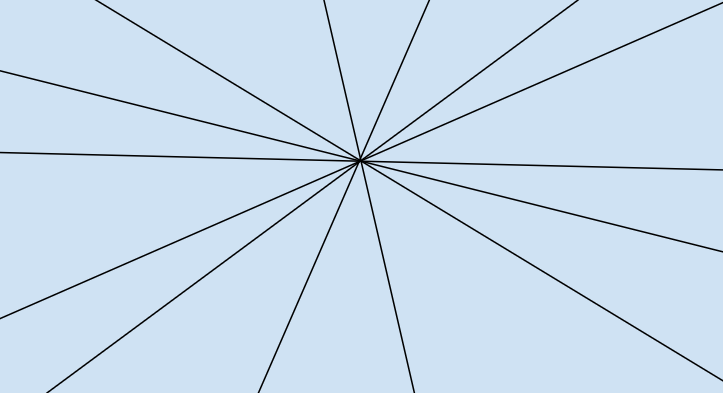
\includegraphics[width = 0.5\linewidth]{images/epipolarlines-a.png}
% \begin{tcolorbox}[colback=white!5!white,colframe=green!75!black]
% \setbox0=\hbox{\parbox[t]{\textwidth}{
%     %%%%%%% ANSWER STARTS HERE %%%%%%%%%%%%%%%%%%%%%%%%%%%%

%     TODO: Your answer to (a) here.

%     %%%%%%% ANSWER ENDS HERE %%%%%%%%%%%%%%%%%%%%%%%%%%%%%%
%     }}
% \clipbox{0pt \dimexpr\dp0-8\baselineskip\relax{} 0in 0pt}{\copy0}
% \end{tcolorbox}

% \item \textbf{[1 point]}
% \begin{tcolorbox}[colback=orange!5!white,colframe=orange!75!black]
% Converge to a point outside of the image plane.
% \end{tcolorbox}

% 
\includegraphics[width = 0.5\linewidth]{images/epipolarlines-b.PNG}

% \begin{tcolorbox}[colback=white!5!white,colframe=green!75!black]
% \setbox0=\hbox{\parbox[t]{\textwidth}{
%     %%%%%%% ANSWER STARTS HERE %%%%%%%%%%%%%%%%%%%%%%%%%%%%

%     TODO: Your answer to (b) here.

%     %%%%%%% ANSWER ENDS HERE %%%%%%%%%%%%%%%%%%%%%%%%%%%%%%
%     }}
% \clipbox{0pt \dimexpr\dp0-8\baselineskip\relax{} 0in 0pt}{\copy0}
% \end{tcolorbox}

% \item \textbf{[1 point]} 
% \begin{tcolorbox}[colback=orange!5!white,colframe=orange!75!black]

% % OLD QUESTION:
% %What might you need to change about your fundamental matrix calculations if you obtained the following epipolar lines?%

% Notice the misalignment of the epipolar lines in the image below? What went wrong in the calculation of the fundamental matrix and how can we fix it?

% \textit{Hint:} Check slides from the lecture on stereo geometry.
% \end{tcolorbox}

% 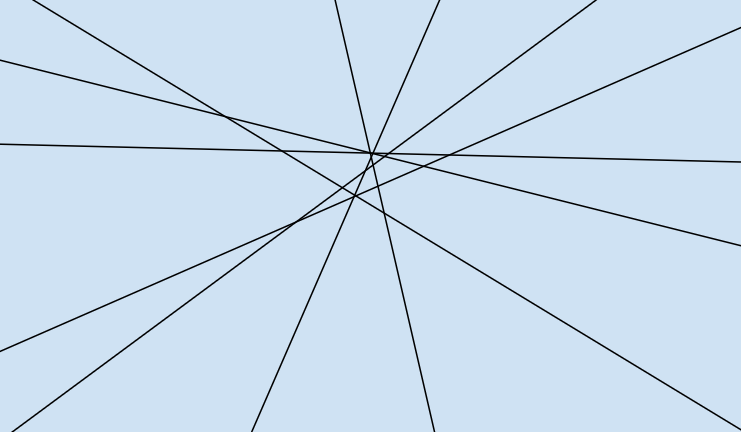
\includegraphics[width = 0.5\linewidth]{images/epipolarlines-c.PNG}
% \begin{tcolorbox}[colback=white!5!white,colframe=green!75!black]
% \setbox0=\hbox{\parbox[t]{\textwidth}{
%     %%%%%%% ANSWER STARTS HERE %%%%%%%%%%%%%%%%%%%%%%%%%%%%

%     TODO: Your answer to (c) here.

%     %%%%%%% ANSWER ENDS HERE %%%%%%%%%%%%%%%%%%%%%%%%%%%%%%
%     }}
% \clipbox{0pt \dimexpr\dp0-8\baselineskip\relax{} 0in 0pt}{\copy0}
% \end{tcolorbox}
% \end{enumerate}



%%%%%%%%%%%%%%%%%%%%%%%%%%%%%%%%%%%
\pagebreak
\section*{Feedback? (Optional)}
Please help us make the course better. If you have any feedback for this assignment, we'd love to hear it!



\end{document}
